              
%%%%%%%%%%%%%%%%%%%%%%%%%%%%%%%%%%%%%%%%%
% Beamer Presentation
% LaTeX Template
% Version 1.0 (10/11/12)
%
% This template has been downloaded from:
% http://www.LaTeXTemplates.com
%
% License:
% CC BY-NC-SA 3.0 (http://creativecommons.org/licenses/by-nc-sa/3.0/)
%
%%%%%%%%%%%%%%%%%%%%%%%%%%%%%%%%%%%%%%%%%

%----------------------------------------------------------------------------------------
%   PACKAGES AND THEMES
%----------------------------------------------------------------------------------------

\documentclass{beamer}

\mode<presentation> {

% The Beamer class comes with a number of default slide themes
% which change the colors and layouts of slides. Below this is a list
% of all the themes, uncomment each in turn to see what they look like.

%\usetheme{default}
%\usetheme{AnnArbor}
%\usetheme{Antibes}
%\usetheme{Bergen}
%\usetheme{Berkeley}
%\usetheme{Berlin}
%\usetheme{Boadilla}
%\usetheme{CambridgeUS}
%\usetheme{Copenhagen}
%\usetheme{Darmstadt}
%\usetheme{Dresden}
%\usetheme{Frankfurt}
%\usetheme{Goettingen}
%\usetheme{Hannover}
%\usetheme{Ilmenau}
%\usetheme{JuanLesPins}
%\usetheme{Luebeck}
\usetheme{Madrid}
%\usetheme{Malmoe}
%\usetheme{Marburg}
%\usetheme{Montpellier}
%\usetheme{PaloAlto}
%\usetheme{Pittsburgh}
%\usetheme{Rochester}
%\usetheme{Singapore}
%\usetheme{Szeged}
%\usetheme{Warsaw}

% As well as themes, the Beamer class has a number of color themes
% for any slide theme. Uncomment each of these in turn to see how it
% changes the colors of your current slide theme.
\usepackage{colortbl}
%\usecolortheme{albatross}
%\usecolortheme{beaver}
%\usecolortheme{beetle}
%\usecolortheme{crane}
%\usecolortheme{dolphin}
%\usecolortheme{dove}
%\usecolortheme{fly}
%\usecolortheme{lily}
%\usecolortheme{orchid}
%\usecolortheme{rose}
%\usecolortheme{seagull}
%\usecolortheme{seahorse}
%\usecolortheme{whale}
%\usecolortheme{wolverine}

%\setbeamertemplate{footline} % To remove the footer line in all slides uncomment this line
%\setbeamertemplate{footline}[page number] % To replace the footer line in all slides with a simple slide count uncomment this line

%\setbeamertemplate{navigation symbols}{} % To remove the navigation symbols from the bottom of all slides uncomment this line
}
\usepackage[english, greek]{babel}
\usepackage{graphicx} % Allows including images
\usepackage{booktabs} % Allows the use of \toprule, \midrule and \bottomrule in tables

%----------------------------------------------------------------------------------------
%   TITLE PAGE
%----------------------------------------------------------------------------------------
\usepackage[utf8]{inputenc}
\selectlanguage{greek}
\title[Γεωγραφική Αναγνώριση Συγγραφέα]{ΑΝΑΠΤΥΞΗ ΜΕΘΟΔΟΛΟΓΙΑΣ ΑΥΤΟΜΑΤΗΣ ΑΝΑΓΝΩΡΙΣΗΣ ΓΕΩΓΡΑΦΙΚΟΥ ΙΔΙΩΜΑΤΙΣΜΟΥ ΤΟΥ ΣΥΓΓΡΑΦΕΑ ΣΕ ΣΥΛΛΟΓΗ ΚΕΙΜΕΝΩΝ ΑΠΟ ΜΕΣΑ ΚΟΙΝΩΝΙΚΗΣ ΔΙΚΤΥΩΣΗΣ } % The short title appears at the bottom of every slide, the full title is only on the title page

\author{Σιμάκης Παναγιώτης} % Your name
\institute[\selectlanguage{english}CEID] % Your institution as it will appear on the bottom of every slide, may be shorthand to save space
{
Πανεπιστήμιο Πατρών \\ Πολυτεχνική Σχολή \\ Τμήμα Μηχανικών Ηλεκτρονικών Υπολογιστών και Πληροφορικής \\ % Your institution for the title page
\medskip
\textit{\selectlanguage{english}simakis@ceid.upatras.gr} % Your email address
}
\selectlanguage{greek}
\date{\today} % Date, can be changed to a custom date

\begin{document}

\begin{frame}
	\titlepage % Print the title page as the first slide
\end{frame}



%----------------------------------------------------------------------------------------
%   PRESENTATION SLIDES
%----------------------------------------------------------------------------------------



%------------------------------------------------
\begin{frame}
		\frametitle{Περιεχόμενα}
		\tableofcontents % Throughout your presentation, if you choose to use \section{} and \subsection{} commands, these will automatically be printed on this slide as an overview of your presentation
\end{frame}
%------------------------------------------------

\begin{frame}
	\frametitle{Εισαγωγή}
	\section{Εισαγωγή}
	Η ραγδαία ανάπτυξη των μέσων κοινωνικής δικτύωσης και συνολικά του παγκόσμιου ιστού έχουν δημιουργήσει τεράστιο όγκο δεδομένων. Η ίδια του η διαχείριση και η εξαγωγή πληροφορίας αποτελεί καθημερινή πρόκληση. Η επιλογή και του γραπτού λόγου για την έκφραση των χρηστών δημιουργεί ακόμα περισσότερες προκλήσεις ως προς την εξαγωγή γνώσεις από το μεγάλο όγκο δεδομένων που αυξάνεται συνεχώς.\\~\\
	Αντικείμενο της παρούσας εργασίας είναι η ανάπτυξη μεθοδολογίας αυτόματης αναγνώρισης γεωγραφικού ιδιωματισμού του συγγραφέα μέσα από συλλογή κειμένων από μέσα κοινωνικής δικτύωσης. Δηλαδή έχοντας ως είσοδο ένα σύνολο κειμένων, το σύστημα αυτό θα είναι σε θέση να δώσει στην έξοδο την γεωγραφική προέλευση του συγγραφέα.
\end{frame}

%------------------------------------------------
\begin{frame}
	\section{Βασικές Έννοιες}
		\frametitle{Βασικές Έννοιες}
		{\Large Εξόρυξης Γνώσης}
		\begin{itemize}
			\item Συσταδοποίηση
			\item Κανόνες συσχέτισης
			\item Κατηγοριοποίηση\linebreak
		\end{itemize}
		{\Large Κατηγοριοποίηση Κειμένου \selectlanguage{english}(Text Categorization)\selectlanguage{greek}}
		\begin{itemize}
			\item Ευρετηριοποίηση Κειμένου \selectlanguage{english}(Document Indexing)\selectlanguage{greek}
			\item Εκπαίδευση κατηγοριοποιητή
		\end{itemize}
\end{frame}
%--------------------------------------
\begin{frame}
	\frametitle{Βασικές Έννοιες}
	\begin{itemize}
		\item {\Large Αναγνώριση Συγγραφέα \selectlanguage{english}(Authorship Attribution)} \selectlanguage{greek}\linebreak
		\item {\Large Αναγνώριση Γεωγραφικού Ιδιωματισμού}
	\end{itemize}
\end{frame}
%--------------------------------------
\begin{frame}
	\section{Εργαλεία Υλοποίησης}
		\frametitle{Εργαλεία Υλοποίησης}
		η υλοποίηση για την εξαγωγή των χαρακτηριστικών έγινε με χρήση της \selectlanguage{english}Python \linebreak
		\begin{itemize}
			\item \selectlanguage{english} {\Large NLTK} (Natural Language ToolKit)\linebreak
			\item \selectlanguage{english} {\Large WEKA} (Waikato Environment for Knowledge Analysis)
		\end{itemize}
		
\end{frame}
%--------------------------------------
\begin{frame}
	\section{Μεθοδολογία}
	\frametitle{Μεθοδολογία}
	για την υλοποίηση της πειραματικής διαδικασίας ακολουθήθηκε η εξής μεθοδολογία:\linebreak
	\begin{enumerate}
		\item Συλλογή Δεδομένων
		\item Προεπεξεργασία/επισημείωση δεδομένων
		\item Εξαγωγή Χαρακτηριστικών
		\item Επιλογή Χαρακτηριστικών
		\item Πειράματα κατηγοριοποίησης
		\item Συμπεράσματα
	\end{enumerate}
\end{frame}
%--------------------------------------
\begin{frame}
	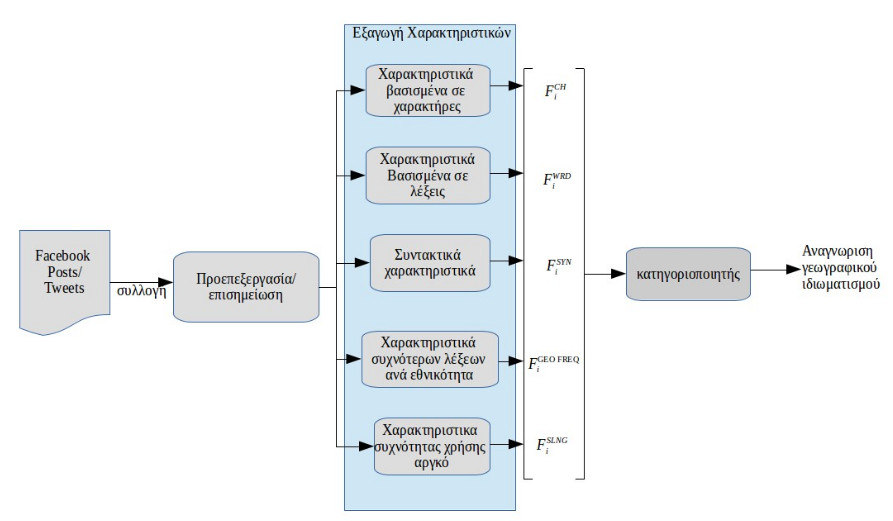
\includegraphics[width=12cm]{img/sys}
\end{frame}
%--------------------------------------
\begin{frame}
	\section{Συλλογή Δεδομένων}
		\frametitle{Συλλογή Δεδομένων}
			η συλλογή κειμένων έγινε μέσα από προσωπικούς λογαριασμούς χρηστών από το \selectlanguage{english}Facebook \selectlanguage{greek}και το \selectlanguage{english}Twitter\linebreak
			\begin{itemize}
				\item Facepager: \selectlanguage{greek}το εργαλείο συλλογής των κειμένων\linebreak
				\item 252.112 κείμενα, 357 διαφορετικοί συγγραφείς\linebreak
				\item 34.969.115 χαρακτηρες και 5.372.512 λέξεις
			\end{itemize}
		
\end{frame}
%--------------------------------------
\begin{frame}
	\section{Προεπεξεργασία/Επισημείωση Δεδομένων}
	\frametitle{Προεπεξεργασία/Επισημείωση Δεδομένων}
	ακριβές πρότυπο επισημειωμένου αρχείου
	\begin{table}\tiny
		\begin{tabular}{l l l l l l l l l l }
			\toprule
			\selectlanguage{english}id \selectlanguage{greek}
			& Κείμενο
			& Φύλο
			& \begin{tabular}{@{}c@{}}Ηλικιακη\\κατηγορία\end{tabular}
			& \begin{tabular}{@{}c@{}}Ακριβής\\ηλικία\end{tabular}
			& \begin{tabular}{@{}c@{}}Κοινωνικό\\δίκτυο\end{tabular}
			& \begin{tabular}{@{}c@{}}Θεματική\\περιγραφή\end{tabular}
			& εθνικότητα
			& \begin{tabular}{@{}c@{}}Επιπλέον\\πληροφορίες\end{tabular}
			\\
			\midrule\selectlanguage{english}
			\selectlanguage{english}1 &  &\selectlanguage{english}F/M & \selectlanguage{english}\begin{tabular}{@{}c@{}}A/B/C/\\D/E/F*\end{tabular} & $ > 14$ & \selectlanguage{english}\begin{tabular}{@{}c@{}}Facebook/\\Twitter\end{tabular} &  & \selectlanguage{english}\begin{tabular}{@{}c@{}}US/CAN/\\UK/AUS/\\NNS\end{tabular} &  \\
			\vdots  & \vdots & \vdots & \vdots & \vdots & \vdots & \vdots  & \vdots  & \vdots\\
			 &  &  &  &  &  &  &  & \\
			\bottomrule
			\selectlanguage{greek}
		\end{tabular}
	\end{table}
		
\end{frame}

%--------------------------------------
\begin{frame}
	\frametitle{Εξαγωγή Χαρακτηριστικών}
	\section{Εξαγωγή Χαρακτηριστικών}
		\begin{itemize}
			\item Βασισμένα σε χαρακτήρες (46 χαρακτηριστικά)\linebreak
			\item Βασισμένα σε λέξεις (8 χαρακτηριστικά)\linebreak
			\item Συντακτικά (13 χαρακτηριστικά)\linebreak
			\item Βασισμένα στο περιεχόμενο (9 χαρακτηριστικά)
				\begin{itemize}
					\item Χαρακτηριστικά συχνότερων λέξεων ανα εθνικότητα
					\item Χαρακτηριστικά συχνότητας χρήσης αργκό ανα εθνικότητα
				\end{itemize}
		\end{itemize}
\end{frame}
%--------------------------------------
\begin{frame}
	\section{Επιλογή Χαρακτηριστικών}
	\frametitle{Επιλογή Χαρακτηριστικών \selectlanguage{english}(Feature Selection)}
	\begin{table}
		\begin{tabular}{l l l}
			\toprule
			\selectlanguage{greek}α/α & \selectlanguage{english}ReliefF score & \selectlanguage{greek}Χαρακτηριστικό \\
			\midrule
			\tiny1 & \tiny$ 0.00329917 $ & \tiny\selectlanguage{greek}Συνολικός αριθμός κεφαλαίων χαρακτήρων ανα αριθμό χαρακτήρων \\
			\tiny2 & \tiny$ 0.00263219 $ & \tiny\selectlanguage{greek}Συνολικός αριθμός μικρών λέξεων ανα σύνολο λέξεων\\
			\tiny3 & \tiny$ 0.00190155 $ & \tinyΣυνολικός αριθμός κενών χαρακτήρων \\
			\tiny4 & \tiny$ 0.00181929 $ & \tinyΜέσο μήκος λέξης\\
			\tiny5 & \tiny$ 0.00175353 $ & \tinyΣυνολικός αριθμός αλφαβητικών χαρακτήρων ανα σύνολο χαρακτήρων\\
			\tiny6 & \tiny$ 0.00149185 $ & \tinyΣυνολικός αριθμός σημείων στίξης ανα σύνολο χαρακτήρων\\
			\tiny7 & \tiny$ 0.00132278 $ & \tinyΣυνολικός αριθμός χαρακτήρων στις λέξεις ανα σύνολο χαρακτήρων\\
			\tiny8 & \tiny$ 0.00108097 $ & \tinyΣυνολικός αριθμός συμβόλων ανα σύνολο χαρακτήρων\\
			\tiny9 & \tiny$ 0.00095305 $ & \tinyΜέσο μήκος πρότασης ανα σύνολο χαρακτήρων\\
			\tiny10 & \tiny$ 0.00086441 $ & \tinyΣυνολικός αριθμός ψηφίων ανα σύνολο χαρακτήρων\\
			\bottomrule
		\end{tabular}
		\caption{Πίνακας κατάταξης των πρώτων 10 χαρακτηριστικών}
	\end{table}
\end{frame}
%--------------------------------------
\begin{frame}
	\section{Αποτελέσματα Κατηγοριοποίησης}
		\frametitle{Αποτελέσματα Κατηγοριοποίησης}
		\begin{table}
			\begin{tabular}{l l l l l l l l}
   		   						\toprule    & \cellcolor[gray]{0.8}\selectlanguage{english}top10
											& \cellcolor[gray]{0.8}\selectlanguage{english}top20
											& \cellcolor[gray]{0.8}\selectlanguage{english}top30
											& \cellcolor[gray]{0.8}\selectlanguage{english}top40
											& \cellcolor[gray]{0.8}\selectlanguage{english}top50
											& \cellcolor[gray]{0.8}\selectlanguage{english}top60
											& \cellcolor[gray]{0.8}\selectlanguage{english}all
											\\
				\midrule\selectlanguage{english}
					\selectlanguage{english}J48 & 52.28 & \textbf{53.88} & 52.24 & 51.23 & 50.31 & 51.26 & 51.30 \\
					\selectlanguage{english}MLP & 47.17 & 51.16 & \textbf{51.20} & 51.11 & 50.07 & 49.36 & 45.01 \\
					\selectlanguage{english}RandomTree & \textbf{55.58} & 55.20 & 50.66 & 46.01 & 41.53 & 40.62 & 40.52 \\
					\selectlanguage{english}REPTree & 50.45 & 53.18 & \text{53.22} & 52.87 & 52.01 & 52.87 & 52.88 \\
					\selectlanguage{english}RBFNetwork & 46.70 & \textbf{49.30} & 48.89 & 48.00 & 48.53 & 47.91 & 48.44\\
					\selectlanguage{english}Bagging & \cellcolor[gray]{0.8}57.96 & \cellcolor[gray]{0.8}\textbf{61.87} & \cellcolor[gray]{0.8}59.61 & \cellcolor[gray]{0.8}58.34 & \cellcolor[gray]{0.8}57.50 & \cellcolor[gray]{0.8}58.34 & \cellcolor[gray]{0.8}58.35 \\
					\selectlanguage{english}Boosting & 46.71 & 47.62 & 47.62 & 47.62 & \textbf{47.78} & 47.62 & 47.62 \\
					\selectlanguage{english}IBk & \textbf{56.34} & 49.08 & 46.52 & 41.57 & 39.08 & 39.05 & 38.88 \\
				\bottomrule
				\end{tabular}
			\caption{Αποτελέσματα κατηγοριοποίησης}
		\end{table}
\end{frame}

%------------------------------------------------
\begin{frame}
	\section{Συμπεράσματα}
	\frametitle{Συμπεράσματα/Προεκτάσεις}
	\begin{itemize}
		\item Εξαγωγή εξειδικευμένων χαρακτηριστικών για αναγνώριση γεωγραφικού ιδιωματισμού
		\begin{itemize}
			\item Βελτιστοποίηση/Εξέλιξη
			\item Βελτίωση των ποσοστών κατηγοριοποίησης\linebreak
		\end{itemize}

		\item Περαιτέρο έρευνα στο πεδίο της αυτόματης αναγνώρισης συγγραφέα βάσει γεωγραφικού προσδιορισμού
	\end{itemize}
	

\end{frame}
%------------------------------------------------
\begin{frame}
	\huge Ερωτήσεις
	
\end{frame}
\begin{frame}
	\frametitle{Άδεια Χρήσης}
	Το παρόν υλικό διατίθεται με τους όρους της άδειας χρήσης Creative Commons Αναφορά, Μη Εμπορική Χρήση Παρόμοια Διανομή 4.01 ή μεταγενέστερη, Διεθνής Έκδοση.\\~\\
	
\includegraphics[width=2cm,keepaspectratio]{img/cc_logo}
\end{frame}

\end{document}
